\documentclass[11pt, a4paper, oneside]{article}
\usepackage{worksheet}

\begin{document}
	
	\makeheader{SAE}{Objektorientierte \hspace{1cm} Programmierung in Python}
	
	\partnertask{Wiederholung: Klassen- und Objektdiagramme}
	
	Ein Café möchte ein digitales Verwaltungssystem entwerfen.
	Erstellen Sie hierfür ein Klassendiagramm\footnote{Sie können für die Diagramme wieder \href{https://draw.io}{draw.io} nutzen.}:
	
	\begin{itemize}
		\item Ein Produkt soll mit Namen, Preis und Beschreibung gespeichert werden.
		Die Methode \texttt{zeigeInfo()} soll die Produktinformationen als Text ausgeben.
		\item Eine Bestellung hat eine Bestellnummer, ein Datum und einen Gesamtpreis.
		Sie soll die Methoden \texttt{berechneGesamtpreis()} und \texttt{zeigeDetails()} haben.
		\item Ein Kunde hat einen Namen, eine Kundennummer und eine Email.
	\end{itemize}

	Entwerfen Sie zusätzlich ein passendes Objektdiagramm für die folgende Situation:
	
	\begin{itemize}
		\item Das Produkt ``Cappucchino'' kostet 3,50€ und hat die Beschreibung ``Espresso mit Milchschaum''.
		\item Die Bestellung mit der Nummer 20240312 wurde am 12.03.2024 aufgegeben und hat eine Gesamtsumme von 7,00€.
		\item Die Kundin ``Lisa Meier'' hat die Kundennummer 1023 und die E-Mail-Adresse\\ ``lisa.meier@email.de''.
	\end{itemize}

	\singletask{Vorstellungsrunde}

	\begin{enumerate}[label=\alph*)]
		\item Schreiben Sie eine Klasse \texttt{Person}, welche die Attribute \texttt{name} und \texttt{alter} besitzt.
		\item Fügen Sie eine Methode \texttt{vorstellen()} hinzu, die eine Begrüßung mit den gespeicherten Attributen ausgibt.
		\item Erstellen Sie zwei konkrete Personen und lassen Sie sie vorstellen.
		\item Schreiben Sie ein Programm, das den Nutzer nach seinem Namen und Alter fragt.
		Lassen Sie das Programm daraus ein Objekt vom Typ \texttt{Person} erstellen und rufen sie die Methode \texttt{vorstellen()} auf.
	\end{enumerate}

	\pagebreak
	
	\singletask{Patientenverwaltung: Implementierung}
	
	Nachdem Sie in der letzten Stunde das Patientenverwaltungssystem für das Krankenhaus geplant haben, soll es nun konkret umgesetzt werden.
	
	Nutzen Sie Ihre erstellten Objekt- und Klassendiagramme und implementieren Sie diese in Python.
	
	\singletask{Brüche in Python\footnotemark}
	\footnotetext{\href{https://inf-schule.de/oop/python/bank/objekteklassen/uebungen}{Klaus Becker \& Heiko Jochum}}
	
	\begin{wrapfigure}[3]{r}{0.25\textwidth}
		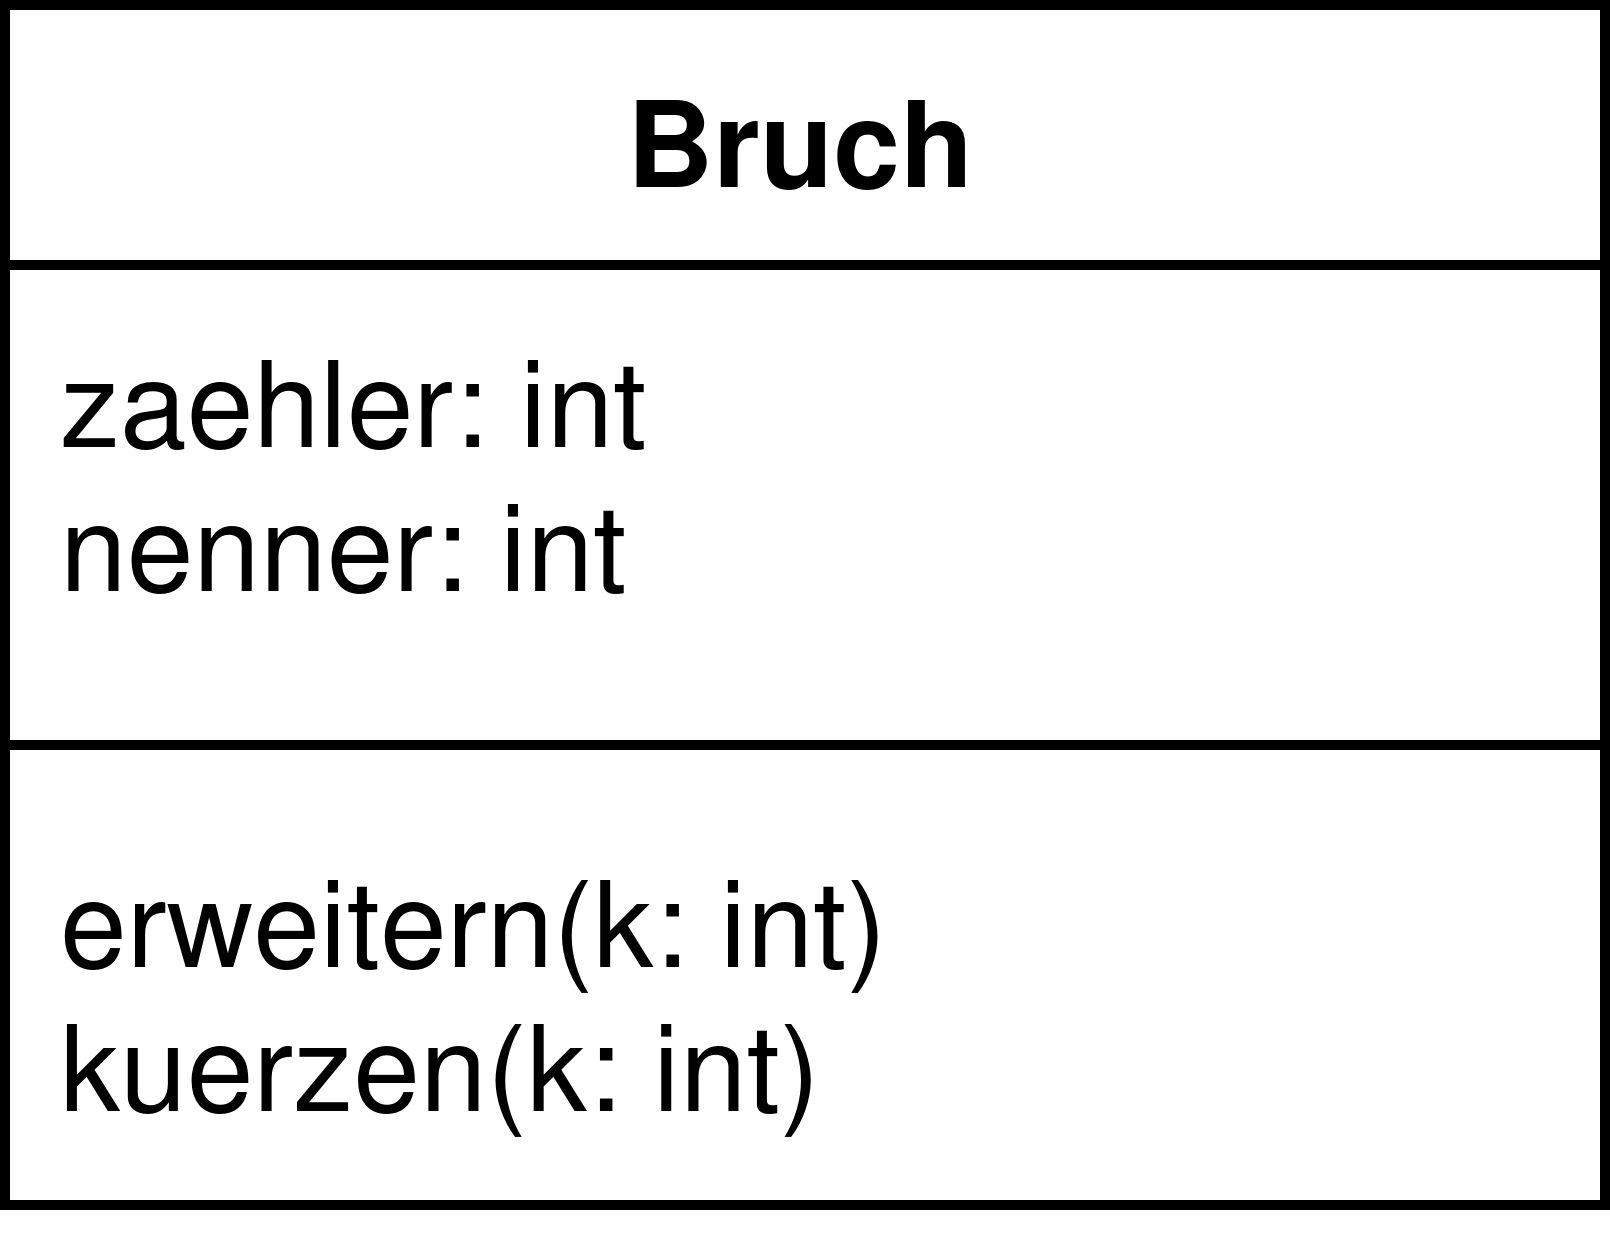
\includegraphics[width=0.25\textwidth]{Bruch.png}
	\end{wrapfigure}

	In Python gibt es keinen Datentyp für Brüche wie $\frac{13}{7}$.
	Implementieren Sie das nebenstehende Klassendiagramm in Python, so dass die folgenden Programmaufrufe möglich werden:
	
	\begin{lstlisting}[language=python, numbers=none]
b = Bruch(4, 6)
b.erweitern(3)
b.kuerzen(2)
b.zaehler
b.nenner
	\end{lstlisting}
	
	Erstellen Sie einige Objekte und Testen Sie das Erweitern und Kürzen der Brüche.
	
	\textbf{Bonus}: Erstellen Sie zusätzlich eine Methode \texttt{vollstaendigKuerzen()} mit entsprechender Implementierung.
	
	\singletask{Zähler\footnotemark[2]}
	
	Ein Zähler ist ein Gerät, mit dem man hochzählen kann, und den man gezielt wieder auf Null setzen kann.
	Man benutzt solche Geräte z.B. bei Verkehrszählungen.
	
	\begin{enumerate}[label=\alph*)]
		\item Modellieren Sie eine Klasse \texttt{Zaehler}, mit der man Objekte erzeugen kann, die sich wie Zähler in der Wirklichkeit verhalten.
		Berücksichtigen Sie vorerst noch nicht, dass es für die Zahl eine Obergrenze gibt.
		Stellen Sie die modellierte Klasse mit einem Klassendiagramm dar.
		Implementieren und testen Sie anschließend die entwickelte Klasse.
		\item Wenn man eine Uhr simulieren möchte, dann benötigt man einen Sekunden- bzw. Minutenzähler, der so zählt:\\
		\texttt{0, 1, 2, 3, ..., 58, 59, 0, 1, 2, 3, ..., 58, 59, 0, 1, 2, ...}\\
		Ein Stundenzähler zählt entsprechend:\\
		\texttt{0, 1, 2, 3, ..., 23, 0, 1, 2, 3, ..., 23, 0, 1, 2, ...}\\
		Modellieren und implementieren Sie auch für Zählsituationen mit einer Obergrenze eine geeignete Klasse.
	\end{enumerate}
	
\end{document}
